\documentclass{beamer}
\usepackage[english]{babel}
\usepackage[utf8]{inputenc}
\usepackage{background}
\usepackage{listings}
\usepackage[orientation=landscape,size=a1]{beamerposter}
\usepackage{tikz}

\usetheme{Warsaw}

\addtobeamertemplate{block begin}{}{\vspace*{20pt}}{}
\addtobeamertemplate{block end}{}{\vspace*{20pt}}

\title{A little survival guide to command line}
\author{Livre Digital Team}
\institute{info@livredigital.com}
\date{\url{https://www.livredigital.com}}

\backgroundsetup{
    placement=center,
    scale=5.15,
    contents={\url{www.livredigital.com}},
    color=black!40,
    angle=25,
    opacity=0.25
}

\setbeamertemplate{background}{\BgMaterial}

\usetikzlibrary{positioning,shadows,arrows}

\linespread{1.25}

% Introduce a new counter for counting the nodes needed for circling
\newcounter{nodecount}
% Command for making a new node and naming it according to the nodecount counter
\newcommand\tabnode[1]{\addtocounter{nodecount}{1} \tikz \node (\arabic{nodecount}) {#1};}
    
\begin{document}
\begin{frame}[t]
    \centering
    \parbox{0.995\textwidth}{    
    \begin{minipage}{.20\linewidth}
        \vspace{20pt}
        \begin{minipage}{0.40\textwidth}
            
\includegraphics[width=\linewidth]{imgs/logo.png}\\
        \end{minipage}
        \begin{minipage}{0.50\textwidth}
            \vspace{20pt}
            Livre Digital\\[0.65cm]
            \small{\emph{We focus our business,\\in open source solutions.}}\\[0.65cm]
            \url{http://www.livredigital.com}
            \vspace{35pt}
        \end{minipage}
    \end{minipage}
    \begin{minipage}[t]{.005\linewidth}
        \hspace{\fill}
    \end{minipage}
    \begin{minipage}{.50\linewidth}
        \vspace{20pt}
        \titlepage
    \end{minipage}
    \begin{minipage}[t]{.055\linewidth}
        \hspace{\fill}
    \end{minipage}
    \begin{minipage}{.20\linewidth}
        Livre Digital, all rights reseved \copyright{} 2017.\\
  \textbf{Licence:} Creative Commons Attribution - Share ALike 4.0\\
  \small{\url{https://creativecommons.org/licenses/by-sa/4.0/legalcode}}
    \end{minipage}
    
    \vspace{20pt}
    
    \begin{center}
    this is a survival guide to all unix users of the world, specially the new ones; this poster have quick tips to use in your day to day life on linux, osx, *bsd.
    \end{center}
    
    \vspace{10pt}
    \hline
    \vspace{10pt}
    
    \begin{minipage}[t]{.25\linewidth}
        \begin{exampleblock}{Top 10 most necessary commands}
        \centering
        \parbox{.95\textwidth}{
        \begin{tabular}{r p{0.35\textwidth} p{0.50\textwidth} }
            \textbf{+} & \textbf{\large description} & \textbf{\large example}\\
            \textbf{pwd} & print working directory & \$ pwd\\
            \textbf{cd} & change directory & \$ cd ..\\
            \textbf{ls} & list files & \$ ls -a *.txt\\
            \textbf{cp} & copy files & \$ cp -rf /dir /opt/subdir\\
            \textbf{mv} & move files & \$ mv oldfile newfilename \\
            \textbf{touch} & creates new file & \$ touch file1 file2\\
            \textbf{mkdir} & creates a directory file & \$ mkdir -pv /tmp/dir/subdir\\
            \textbf{rm} & remove files & \$ rm -f /tmp/file\\
            \textbf{echo} & echoes a line & \$ echo "hello world" \textgreater{} file.txt\\
            \textbf{cat} & concatenate/print files & \$ cat /etc/passwd\\
        \end{tabular}
        \vspace{20pt}
        }
        \end{exampleblock}
        
        \begin{center}
        \p{\textbf{Working with files and directories}}
        \end{center}
        
        \begin{tabular}{l p{9cm} }
        \textbf{\$ cd} & go to the user home directory\\
        \textbf{\$ cd /etc} & enter in the directory etc of /\\
        \textbf{\$ cd /etc/nginx} & enter in the directory nginx of /etc\\
        \textbf{\$ cd ..} & comes back one level up to /etc\\
        \textbf{\$ ls /tmp/*.txt} & list all .txt files in /tmp\\
        \textbf{\$ ls -a /home/user} & list all hidden files of /home/user\\
        \textbf{\$ cp file1 copyfile} & copies a single file\\
        \textbf{\$ cp file1 file2 /tmp} & copies multiple files to /tmp\\
        \textbf{\$ cp file1 copyfile} & copies a single file\\
        \textbf{\$ cp -r ./dir1/ /tmp} & copies recursively dir1 to /tmp\\
        \textbf{\$ mv oldfile newname} & renames oldfile to newname\\
        \textbf{\$ mv file1 file2 /tmp} & moves file1 and file2 to /tmp\\
        \textbf{\$ rm -f /tmp/share.txt} & removes share.txt from /tmp dir\\
        \textbf{\$ rm -rf /tmp/lz0} & removes lz0 subdir from /tmp dir\\
        \textbf{\$ head -n 20 file.txt} & shows first 20 lines of file.txt\\
        \textbf{\$ tail file.txt} & shows last 10 lines of file.txt\\
        \textbf{\$ less file.txt} & shows contents of file.txt pagined\\
        \end{tabular}
        
        \vspace{10pt}
        
        \begin{center}
        \p{\textbf{Process Management, Modifying, Compressing, Archiving}}
        \end{center}
        
        \begin{tabular}{l p{9cm} }
        \textsc{process management} &\\
        \textbf{\$ top} & interactive display of processes\\
        \textbf{\$ ps aux} & show all users processes of system\\
        \textbf{\$ kill -9 10002} & kill a process id (PID) number 10002\\
        \textbf{\$ nice -n -10 2553} & give a better priority for pid 2553\\
        \textsc{(de)compression} & \small \textbf{c:} create; \textbf{t:} contents; \textbf{j:} bzip; \textbf{z:} gzip\\
        & \textbf{x:} extract; \textbf{v:} verbose; \textbf{r:} recursive\\
        \textbf{\$ tar cvfz /usr /var file.tar.gz} & compress /usr and /var into file.tar.gz\\
        \textbf{\$ tar xfj file.tar.bz2 -C /opt} & extract file.tar.bz2 into /opt\\
        \textbf{\$ zip -r /tmp temporary.zip} & compress /tmp dir into temporary.zip\\
        \textbf{\$ gzip /var/log/messages} & compress messages file into .gz\\
        \textsc{install source files} &\\
        \textbf{\$ ./configure \&\& make} & check dependencies, build software\\
        \textbf{\$ make install} & install software for all users
        \end{tabular}

    \end{minipage}
    \begin{minipage}[b]{.010\linewidth}
        \hspace{\fill}
    \end{minipage}
    \begin{minipage}[t]{.50\linewidth}
        \begin{block}{The VI / VIM editor}
        \centering
        \parbox{.95\linewidth}{
        \begin{minipage}[t]{0.475\textwidth}
            The VI editor is probably the most used editor in UNIX systems, it comes with almost any distribution of Linux,
            *BSD and can be also used in OSX. The editor comes with
            two main modes: command and insertion.\\
            
            The insertion mode is commonly to all users, you just
            type something and text typed will be into file, the command mode is accessed by hotkey \textbf{[ESC]}
            
            \vspace{10pt}
            
            \begin{tabular}{r p{14cm} }
                \textbf{hotkey} & \textbf{description}\\
                \textbf{h, j, k, l} & move cursor left, down, top, right respectively\\
                \textbf{0, \$} & move cursor to the beginning and end of line respectively\\
                \textbf{u, [ctrl] + r} & (u)ndo last and redo last change respectively\\
                255\textbf{G, G} & go to line 255, go to last line respectively\\
                \textbf{i, o} & go to (i)nsert mode, insert on next line respectively\\
            \end{tabular}
        \end{minipage}
        \begin{minipage}[t]{0.010\textwidth}
            \hspace{\fill}
        \end{minipage}
        \begin{minipage}[t]{0.470\textwidth}
            There are many others commands in VI, some of these starts
            with colons (\textbf{:}), here are some of the most used 
            in our opinion:
            \vspace{10pt}
            
            \begin{tabular}{r p{14cm} }
                \textbf{command} & \textbf{description}\\
                \textbf{:w, :wq} & (w)rite file, (w)rite file and (q)uit file.\\
                \textbf{:q, :q!} & quit file, or quit file without change anything\\
                \textbf{:!gcc file.c} & executes gcc to compile file.c into ./a.out binary\\
                \textbf{:r !date} & read the output of command \textit{date} and puts on file\\
                \textbf{:set number} & show line numbers at left\\
                \textbf{:5,20d} & delete lines 5 - 20\\
                \textbf{:\%s/old/new/g} & replaces all occurrences of \textit{old} to \textit{new} string\\
                \textbf{:help cmd} & get help about cmd\\
                \textbf{:vimtutor} & starts the tutorial mode for learning vi\\
            \end{tabular}
        \end{minipage}
        }
        \end{block}
    
        \begin{center}
        \textbf{Basic Systems and Network Management Commands}
        \end{center}
        
        \vspace{10pt}
        
        \begin{minipage}[t]{0.475\textwidth}
            \begin{tabular}{l p{10cm} }
            \textbf{\$ dmesg} & display system messages from kernel\\
            \textbf{\$ fdisk} & manage disk partitions table\\
            \textbf{\$ fsck /dev/sda} & check and repair filesyste, /dev/sda\\
            \textbf{\$ groupadd dev} & creates dev group (groupdel removes)\\
            \textbf{\$ lsmod} & list all modules loaded by kernel\\
            \textbf{\$ mkfs -t ext4 /dev/disk} & format /dev/disk with ext4 fs\\
            \textbf{\$ mkswap /tmp/file} & setup a swap area for use\\
            \textbf{\$ mount /dev/sdc1 /mnt} & maps device /dev/sdc1 on /mnt\\
            \textbf{\$ passwd billy} & modifies the password of user billy\\
            \textbf{\$ shutdown (-r/-h) now} & reboot, halts the system at specified time\\
            \textbf{\$ umount /mnt} & unload the device mapped on /mnt dir\\
            \textbf{\$ useradd joe} & add user joe to system (userdel removes)\\
            \end{tabular}
        \end{minipage}
        \begin{minipage}[t]{0.010\textwidth}
            \hspace{\fill}
        \end{minipage}
        \begin{minipage}[t]{0.470\textwidth}
            \begin{tabular}{l p{11cm} }
            \textbf{\$ ping livredigital.com} & pings a hostname or ip\\
            \textbf{\$ ifconfig -a} & show interface(s) network information\\
            \textbf{\$ route -n} & displays, add and del gateway on network\\
            \textbf{\$ iptables -L -n -v} & display the firewall rules\\
            \textbf{\$ traceroute google.com} & display the nr of hops to reach google\\
            \textbf{\$ netstat -nap} & display (A)LL socket connections\\
            \textbf{\$ dig livredigital.com} & query all DNS records for host\\
            \textbf{\$ host google.com} & get the ip address of host\\
            \textbf{\$ whois domain.com} & get the registry records for domain\\
            \textbf{\$ tcpdump -i eth0 -vv} & sniff all packets of eth0 interface\\
            \textbf{\$ nc 10.0.0.1 25} & a really powerful tool for network test\\
            \textbf{\$ ssh root@google.com} & remote connect on console of a network host\\
            \end{tabular}
        \end{minipage}
        
        \vspace{10pt}
        
        \begin{center}
        \textbf{Distribution Package Management - Search, Installs, Remove Packages}
        \end{center}
        
        \begin{minipage}[t]{0.475\textwidth}
        \begin{alertblock}{Red Hat Linux - YUM and RPM}
            \vspace{10pt}
            \centering
            \parbox{.95\textwidth}{
            \begin{tabular}{r | p{0.40\textwidth} p{0.40\textwidth} }
                \textbf{} & \textbf{\large description} & \textbf{\large example}\\
                \hline
                \textbf{yum} & \multicolumn{2}{l}{the yum software package manager} \\
                \multicolumn{2}{r}{update metadata of repository} & \# yum update\\
                \multicolumn{2}{r}{upgrade all packages} & \# yum upgrade\\
                \multicolumn{2}{r}{search for vim rpm on repository} & \# yum search vim\\
                \multicolumn{2}{r}{install dependencies and the package} & \# yum install vim\\
                \textbf{rpm} & \multicolumn{2}{l}{red hat package manager}\\
                \multicolumn{2}{r}{install a rpm package} & \# rpm -ivh file.rpm\\
                \multicolumn{2}{r}{list all rpm's installed on system} & \# rpm -qa\\
                \multicolumn{2}{r}{shows the rpm package relative to file} & \# rpm -qf /usr/bin/ls\\
                \multicolumn{2}{r}{shows file contents of package} & \# rpm -ql file.rpm\\
                \multicolumn{2}{r}{remove redhat package} & \# rpm -ev file.rpm\\
            \end{tabular}
            \vspace{20pt}
            }
        \end{alertblock}
        \end{minipage}
        \begin{minipage}[t]{0.045\textwidth}
            \hspace{\fill}
        \end{minipage}
        \begin{minipage}[t]{0.475\textwidth}
        \begin{exampleblock}{Debian GNU/Linux}
            \vspace{10pt}
            \centering
            \parbox{.95\textwidth}{
            \begin{tabular}{r | p{0.40\textwidth} p{0.36\textwidth} }
                \textbf{} & \textbf{\large description} & \textbf{\large example}\\
                \hline
                \textbf{apt-get} & \multicolumn{2}{l}{the apt software package manager} \\
                \multicolumn{2}{r}{update metadata of repository} & \# apt-get update\\
                \multicolumn{2}{r}{upgrade all installed pkgs} & \# apt-get upgrade\\
                \multicolumn{2}{r}{install dependencies and the package} & \# apt-get install vim\\
                \textbf{apt-cache} & \multicolumn{2}{l}{browse packages on repository} \\
                \multicolumn{2}{r}{show basic information of a pkg} & \# apt-cache show pkgname\\
                \multicolumn{2}{r}{show dependencies of pkgname} & \# apt-cache depends pkg\\
                \multicolumn{2}{r}{search for ncurses .deb on repository} & \# apt-cache search ncurses\\
                \textbf{dpkg} & \multicolumn{2}{l}{debian package manager}\\
                \multicolumn{2}{r}{install a deb package} & \# dpkg -i file.deb\\
                \multicolumn{2}{r}{list all deb's installed on system} & \# dpkg -l\\
                \multicolumn{2}{r}{remove a deb's installed package} & \# dpkg -r file.deb\\
                \multicolumn{2}{r}{shows the contents of deb package} & \# dpkg -c file.deb\\
            \end{tabular}
            \vspace{20pt}
            }
        \end{exampleblock}
        \end{minipage}
    \end{minipage}
    \begin{minipage}[b]{.010\linewidth}
        \hspace{\fill}
    \end{minipage}
    \begin{minipage}[t]{.23\linewidth}
        \begin{exampleblock}{ UNIX Directory Structure Tree }
            \vspace{10pt}
            \centering
            \begin{tikzpicture}[
                fact/.style={rectangle, draw=none, rounded corners=1mm, fill=black, drop shadow, text centered, anchor=north, text=white},
                state/.style={rectangle, draw=none, fill=gray, circular drop shadow, text centered, anchor=north, text=white},
                level distance=1.25cm, growth parent anchor=south
            ]
            \node (State00) [state] {/} [->, sibling distance=2.25cm]
                child { node (Fact01) [fact] {/bin} }
                child { node (Fact10) [fact] {/dev} }
                child {[sibling distance=3.5cm] node (Fact02) [fact] {/etc}
                    child{ node (leaf01) [state] {/etc/passwd} }
                    child{ node (leaf02) [state] {/etc/nginx} }
                }
                child {[sibling distance=5cm] node (Fact03) [fact] {/home} }
                child {[sibling distance=5cm] node (Fact04) [fact] {/lib} }
                child {[sibling distance=5cm] node (Fact04) [fact] {/sbin} }
                child {[sibling distance=3.5cm] node (Fact05) [fact] {/var}
                    child{ [sibling distance=5cm] node (State03) [state] {/var/log}
                        child{ [sibling distance=13cm] node (Fact07) [fact] {/var/log/nginx} } }
                    child{ [sibling distance=3cm] node (State04) [state] {/var/run} }
                }
             ;
            \end{tikzpicture}

            \parbox{.9\textwidth}{
            \begin{minipage}[t]{0.5\linewidth}
                \begin{tabular}{r p{0.65\textwidth}}
                \textbf{\large dir} & \textbf{\large description}\\
                \textbf{/} & root directory\\
                \textbf{/bin} & binary files\\
                \textbf{/dev} & device and peripheral\\
                \textbf{/etc} & system config files\\
                \textbf{/home} & users directory\\
                \end{tabular}
            \end{minipage}
            \begin{minipage}[b]{0.5\linewidth}
                \begin{tabular}{r p{0.8\textwidth}}
                & \\
                \textbf{/lib} & libraries and kernel modules\\
                \textbf{/opt} & optional softwares\\
                \textbf{/sbin} & super binary files\\
                \textbf{/usr} & programs shareable content\\
                \textbf{/var} & temporary/log files\\
                \end{tabular}
            \end{minipage}
            \vspace{10pt}
            }
        \end{exampleblock}
        
        \vspace{10pt}
        
        \parbox{.95\textwidth}{
        \begin{itemize}
            \item Structured hierarchy directory;
            \item Everything is a file and they are case sensitive;;
        \end{itemize}
        
        % \vspace{10pt}
        
        % \begin{tabular}{r p{6cm}}
        %     \textsc{absolute path} & /var/log/nginx/access\_log\\
        %     \textsc{relative path} & ./nginx/access\_log
        % \end{tabular}
        }
        
        \vspace{10pt}

        \begin{block}{UNIX Permissions}
        \centering
        \parskip -1.5mm
        \parbox{.95\textwidth}{
            \textbf{\$ cd /etc; ls -lhd passwd profile* rc.local resolv*}\\
            \smallsize{(list passwd, rc.local and all other files starting
            by prefix 'profile' and 'resolv')}\\
            \begin{tabular}{c c l l r l r l}
            \smallsize
            & & & & & & & \\
            -rw-r--r-- & 1 & root & root &   1.9K & May 24 & 18:43 & passwd\\
            -rw-r--r-- & 1 & root & root    & 761 & Oct 22 &  2014 & profile\\
            drwxr-xr-x & 2 & root & root   & 4.0K & Feb 10 & 17:56 & profile.d\\
            -rwxr-xr-x & 1 & root & admin  & 306 & Feb 10 & 17:49 & rc.local\\
            -rw-r--r-- & 1 & root & root    & 935 & May 12 & 23:41 & resolv.conf\\
            \end{tabular}
            
            \vspace{20pt}
            
            \$ ls -l rc.local\\
            -rwxr-xr-x & 1 & root & admin  & 306 & Feb 10 & 17:49 & rc.local
            
            \vspace{15pt}
            
            
            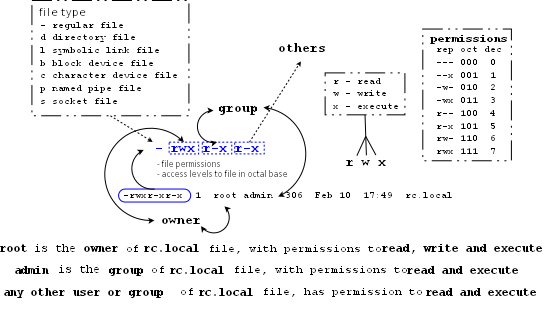
\includegraphics[width=1.045\linewidth]{imgs/unix_perm.png}
            
            {\raggedright
                \textbf{\$ chmod ug+wx rc.local}\\
                \smallsize{change permission to (u)ser, (g)roup of (w)rite and e(x)ecute}\\
                \textbf{\$ chmod o-rwx rc.local}\\
                \smallsize{removes all permissions (read, write, execute) to any other user/group}\\
            }
            \vspace{10pt}
            }
        \end{block}
    \end{minipage}
    % \begin{minipage}[t]{.005\linewidth}
    %     \hspace{\fill}
    % \end{minipage}
    }
\end{frame}
\end{document}